A distinction exists between \ac{PV} cell, panel/module, and the \ac{SA} surface area. \ac{PV} cells are interconnected together in a package called a panel, or module, which is then wired in series and parallel into a \ac{PV} array. The interconnections between cells and wiring between panels introduce cell coverage gaps from which no power is generated. As such, considering panel or array rather than cell surface area for power and energy calculations would result in over-estimated values. By way of example, \refFig{fig:image:mer-solar-arrays} presents the \ac{MER} Opportunity \ac{SA} which is made up of a total of 499 cells: 165 on the port wing, 167 on the starboard wing, 102 on the stern, and 65 on the body. A cell's dimension is $\SI{3.95}{\centi\meter} \times \SI{6.89}{\centi\meter}$ with two cropped corners. This provides an active area of \SI{26.6}{\centi\meter\squared} thus the solar cell coverage area is $499 \times \SI{26.6}{\centi\meter\squared} = \SI{1.3}{\meter\squared}$.

%\todo[inline]{\text{TODO:} Source E-mail exchange with Richard C. Ewell (NASA/JPL) for the MER solar cell size.}

\begin{figure}[h]
\captionsetup[subfigure]{justification=centering}
%\vspace{-2ex}
\centering
    %% setup sizes
    \setlength{\subfigureWidth}{0.50\textwidth}
    \setlength{\graphicsHeight}{60mm}
    %% kill hyper-link highlighting
    \hypersetup{hidelinks=true}%
    %% the figures
    \begin{subfigure}[t]{\subfigureWidth}
        \centering
            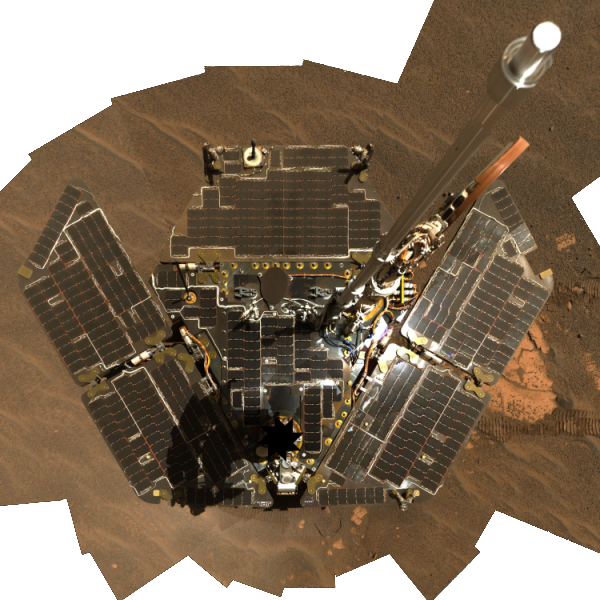
\includegraphics[height=\graphicsHeight]{sections/mars-solar-energy/photovoltaic-energy/images/mer-solar-arrays.png}
            \subcaption{Solar array}
            \label{fig:image:mer-solar-arrays}
    \end{subfigure}\hfill
    \begin{subfigure}[t]{\subfigureWidth}
        \centering
            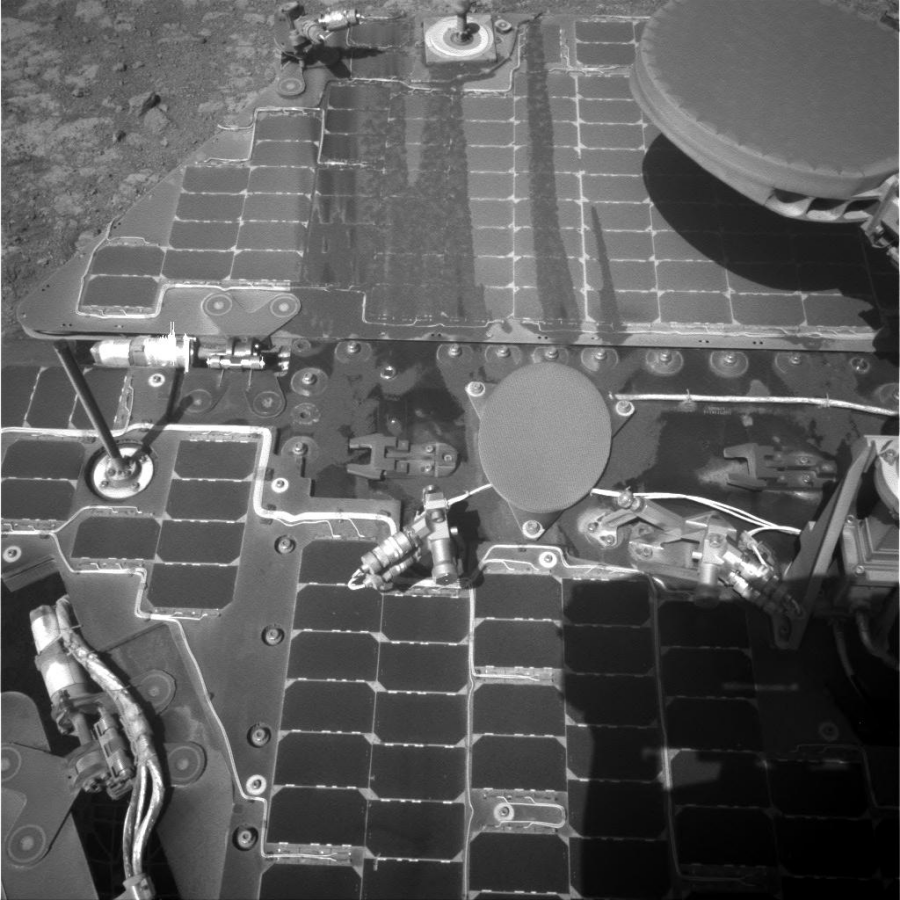
\includegraphics[height=\graphicsHeight]{sections/mars-solar-energy/photovoltaic-energy/images/mer-opportunity-dust-streaks.png}
            \subcaption{Dust streaks}
            \label{fig:image:mer-opportunity-dust-streaks}
    \end{subfigure}\\[0.8ex]
    \caption[Opportunity solar arrays and dust streaks]
    {Opportunity \acp{SA} and dust streaks. (a) Solar arrays. Image: \ac{NASA}/\ac{JPL}-Caltech/Cornell. (b) During a forward, uphill drive on Sol 4311 (March 10, 2016), Opportunity's tilt reached \SI{32}{\degree}. Vibrations from wheels slipping against the ground caused dust to streak down from \ac{MER} Opportunity's rear solar array while the rover was steeply tilted. Image taken on Sol 4322 (March 21, 2016). Image: \ac{NASA}/\ac{JPL}-Caltech.}
    \label{fig:mer-solar-arrays-and-dust-streaks}
\vspace{-2ex}
\end{figure}

% Solar array source: https://mars.nasa.gov/resources/5852/opportunity-self-portrait/?site=insight

% Dust streak source: https://www.nasa.gov/feature/jpl/rover-takes-on-steepest-slope-ever-tried-on-mars


\subsection{Performance Ratio}
\label{sec:PowerAndEnergyPredictions:PerformanceRatio}
Power and energy calculations take into account solar cell \ac{PR}, also known as the coefficient for losses. \ac{PR} components are taken from Mars \ac{PV} literature:

\begin{enumerate}[label=\textcolor{BulletBlue}{(\alph*)}]
  \item\label{itm:pr:perm_loss}After deployment, \SI{5}{\percent} permanent dust power loss \citepower{McNatt2016}.
  \item\label{itm:pr:temp}Solar cell efficiency varies by \SI{3}{\percent} due to changing temperature and red-shift spectral losses through the day time-period \citepower{Kerslake1999}.
  \item\label{itm:pr:deposition}Dust deposition degrades the performance at a rate of \SI{0.28}{\percent} per sol during the initial 30 Sols of a mission and long-term degradation is about \SI{0.14}{\percent} per sol \citepower{Landis2004}.
  \item\label{itm:pr:saturation}Dust performance degradiation saturates at about \SI{30}{\percent} \citepower{Stella2005}.
  \item\label{itm:pr:shadowing}Variable shadowing from protruding rover structures \citepower{Stella2005} and terrain masking \citepower{Kerslake1999}.
\end{enumerate}

%The \ac{PR} in the daily energy calculations throughout this chapter are partly made up of degradation coefficients from \ref{itm:pr:perm_loss} and \ref{itm:pr:temp}. Validation against \ac{MER} Opportunity data uses the \ac{SA} dust factor reported by the rover rather than those described in \ref{itm:pr:deposition} and \ref{itm:pr:saturation}. Losses from \ref{itm:pr:shadowing} and other unaccounted factors are first assumed at \SI{5}{\percent} before iteratively revising them along with \ac{SA} dust factor so that the error margin range may be reduced.

Dust deposition induced losses do not perennially degrade the solar cells but fluctuate due to probabilistic dust cleaning events such as encounters with dust devils, storm winds, or even from a steep tilt angle as seen in \refFig{fig:image:mer-opportunity-dust-streaks}.

\subsection{Predictions}
\label{sec:PowerAndEnergyPredictions:Predictions}

The power output $P$ generated from a photovoltaic system is measured in Watts (\si{\watt}) and is obtained from the global irradiance $G_{h}$ captured by its solar cells:

\begin{equation}
  \label{eq:SA_power}
  P = A \cdot \eta \cdot G_{h} \cdot PR
\end{equation}

where $A$ is the solar cell coverage area $\eta$ their efficiency.

The generated daily energy output $E$ is measured in Watt-hours (\si{\watt\hour}) and is obtained from the daily global insolation $H_{h}$ captured by solar cells:

\begin{equation}
  \label{eq:SA_energy}
  E = A \cdot \eta \cdot H_{h} \cdot PR
\end{equation}

Power and energy calculations for inclined solar arrays are obtained from $G_{\beta}$ and $I_{\beta}$. They are denoted as $P_{\beta}$ and $E_{\beta}$ respectively:

\begin{equation}
  \label{eq:SA_slope_power}
  P_{\beta} = A \cdot \eta \cdot G_{\beta} \cdot PR
\end{equation}


\begin{equation}
  \label{eq:SA_slope_energy}
  E_{\beta} = A \cdot \eta \cdot H_{\beta} \cdot PR
\end{equation}

\subsection{Validation}
\label{sec:PowerAndEnergyPredictions:Validation}
%\todo[inline]{\textbf{TODO:} Write section introduction.}

%\todo[inline]{TODO: Short intro text? Why are we validating? Explain that the equations we are using were based on Viking Lander data and we need to verify if it is still robust today by validating it against the wealth of data we've accumulated since, specifically with MER Opportunity data which is illustrative of mobile rover missions rather than a stationary lander mission.}

\subsubsection{Horizontal Surface}
\label{sec:PowerAndEnergyPredictions:Validation:HorizontalSurface}

In order to validate the formulas presented in \refSec{sec:PowerAndEnergyPredictions:Predictions}, \ac{MER} Opportunity status update parameters are applied to the daily energy calculation presented in \refEqn{eq:SA_energy}. The following data is scraped from the rover's status update website for Mars years \ac{MY}29 through \ac{MY}33:

\begin{enumerate}[label=\textcolor{BulletBlue}{(\alph*)}]
  \item Sol: the mission's Martian day when the status report was made.
  \item Terrestrial date: the date on Earth when the status report was made.
  \item Atmospheric opacity: the $\tau$ factor introduced in  \refSec{sec:MartianEnvironment:Dust:AtmosphericOpacity}.
  \item \ac{SA} dust factor: a value between 0 and 1 with the latter represents perfectly clean \acp{SA}.
  \item Daily energy production: in Watt-hours (\si{\watt\hour}).
\end{enumerate}

For the purpose of insolation calculations, the areocentric longitude $L_{s}$ is determined from the terrestrial date based on the process and equations in \citeother{Allison2000}. The resulting predicted energy production is then compared to the rover's reported daily energy production. These are presented for selected Mars years in \refFig{fig:plot:mer-energy-production-predicted-vs-reported}. A clear outlier is observed during the second half of \ac{MY}33 in which predicted daily energy productions are much higher than reported. This is due to the rover's inclined descent through ``Bitterroot Valley'' during an intensive investigation into a gully at Endeavour Crater's western rim. Energy production predictions with horizontal surface \refEqn{eq:SA_energy} not suited due to the inclination and orientation of such a descent. Applying \refEqn{eq:SA_slope_energy} for $E_{\beta}$ would be more applicable. As such, data from \ac{MY}33 is not considered in the validation exercise for horizontal surfaces.

\begin{figure}[h]
\captionsetup[subfigure]{justification=centering}
%\vspace{-2ex}
	\centering
    %% setup sizes
    \setlength{\subfigureWidth}{0.50\textwidth}
    \setlength{\graphicsHeight}{70mm}
    %% kill hyper-link highlighting
    \hypersetup{hidelinks=true}%
    %% the figures
%% 1st row
  	\begin{subfigure}[t]{\subfigureWidth}
      \centering
  		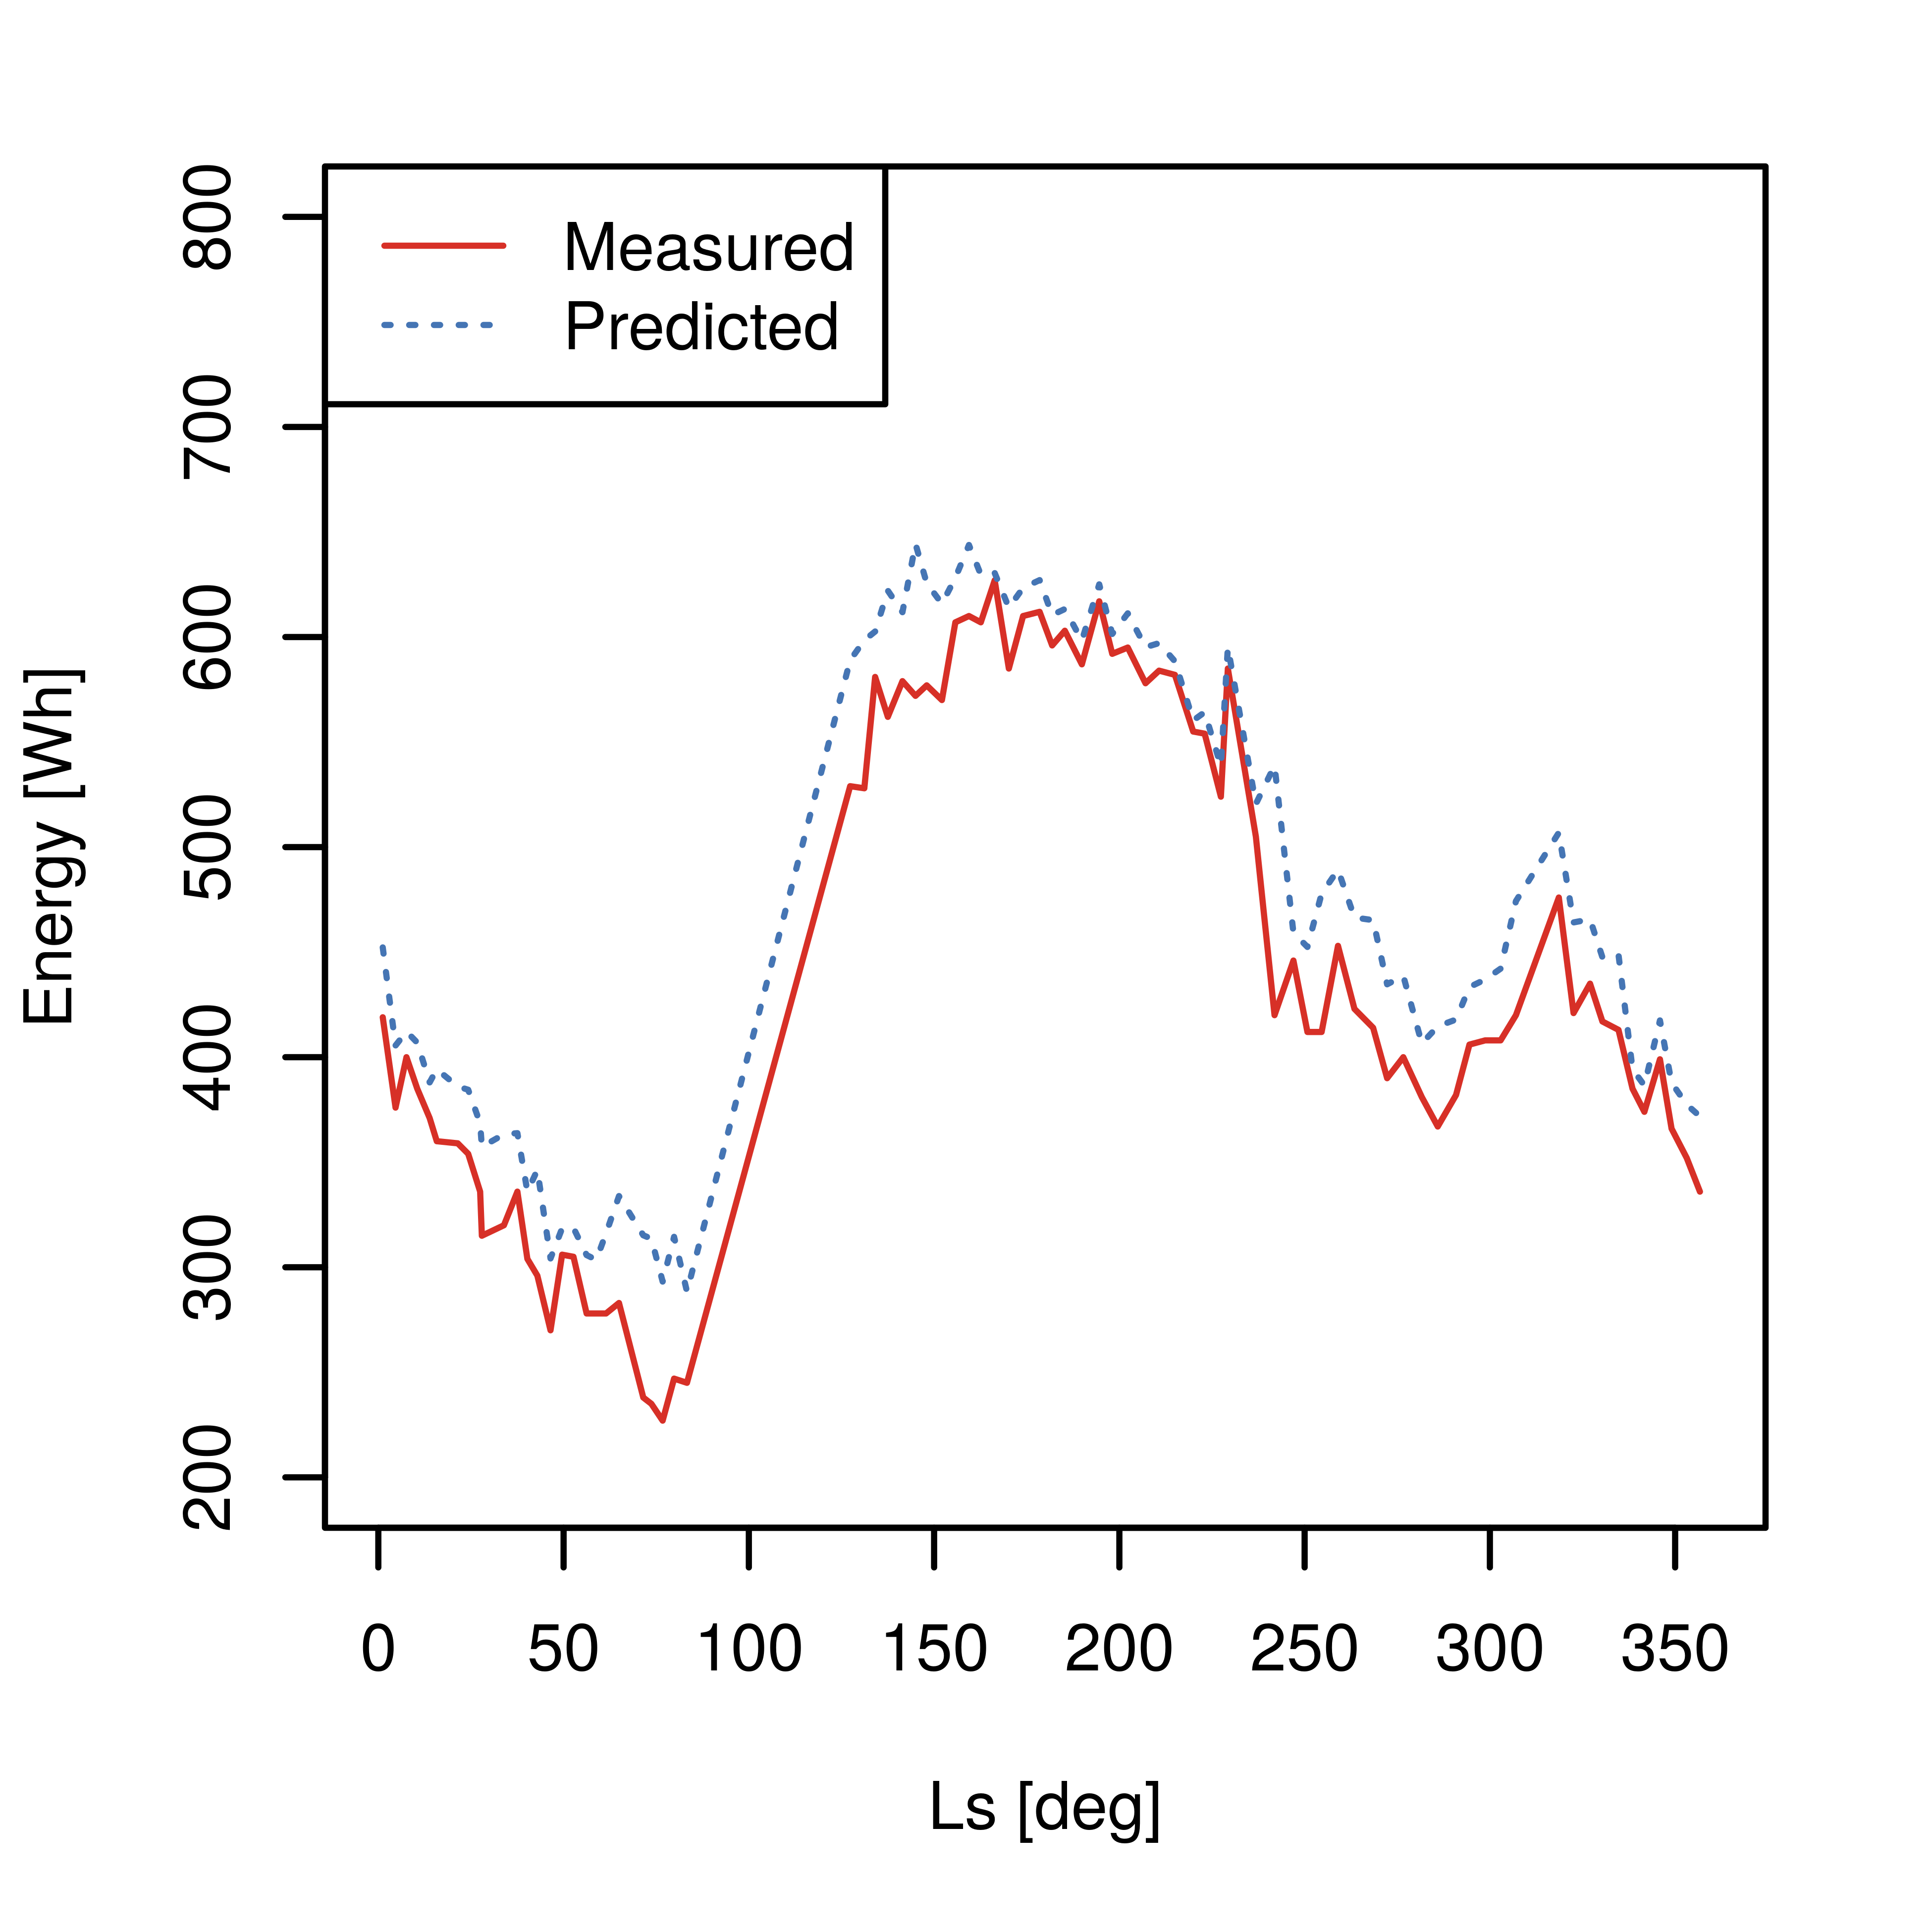
\includegraphics[height=\graphicsHeight]{sections/mars-solar-energy/photovoltaic-energy/plots/predicted-vs-measured-energy-my29.png}
  		\subcaption{MY29}
  		\label{fig:plot:sub:mer-energy-production-predicted-vs-reported-my29}
  	\end{subfigure}\hfill
    \begin{subfigure}[t]{\subfigureWidth}
      \centering
  		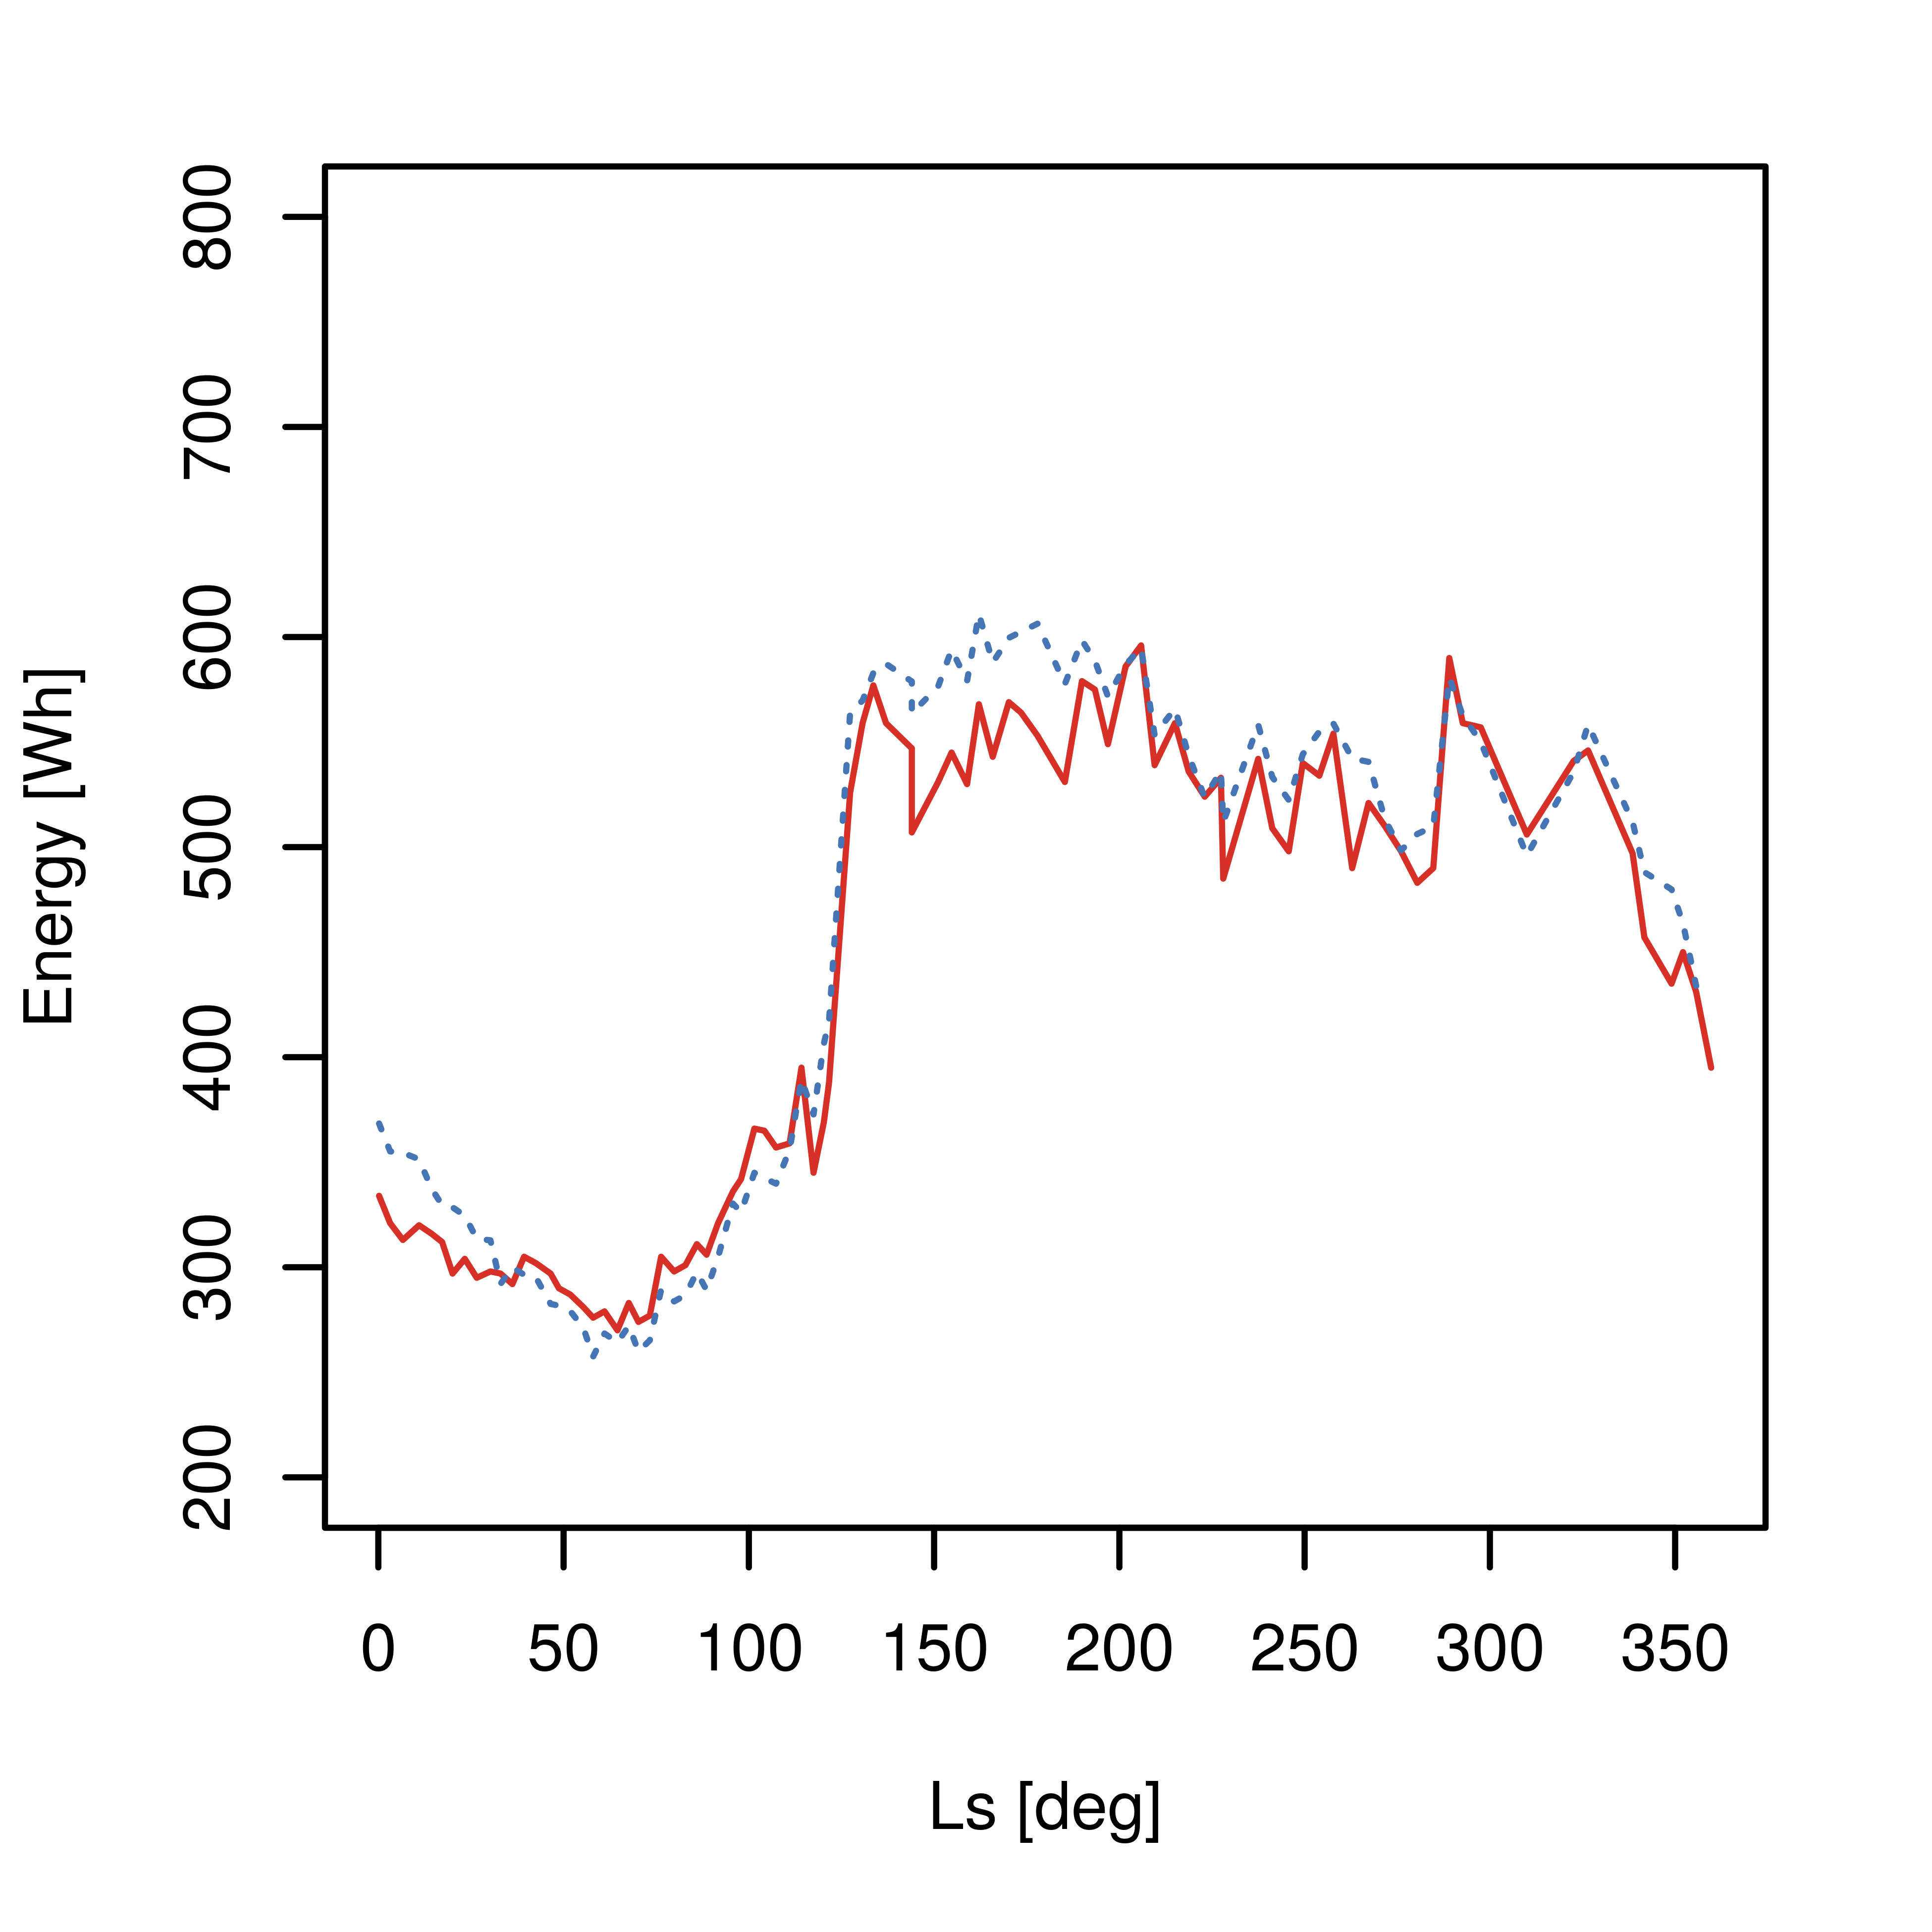
\includegraphics[height=\graphicsHeight]{sections/mars-solar-energy/photovoltaic-energy/plots/predicted-vs-measured-energy-my30.png}
  		\subcaption{MY30}
  		\label{fig:plot:sub:mer-energy-production-predicted-vs-reported-my30}
  	\end{subfigure}\\[0.8ex]
%% 2nd row
    \begin{subfigure}[t]{\subfigureWidth}
      \centering
  		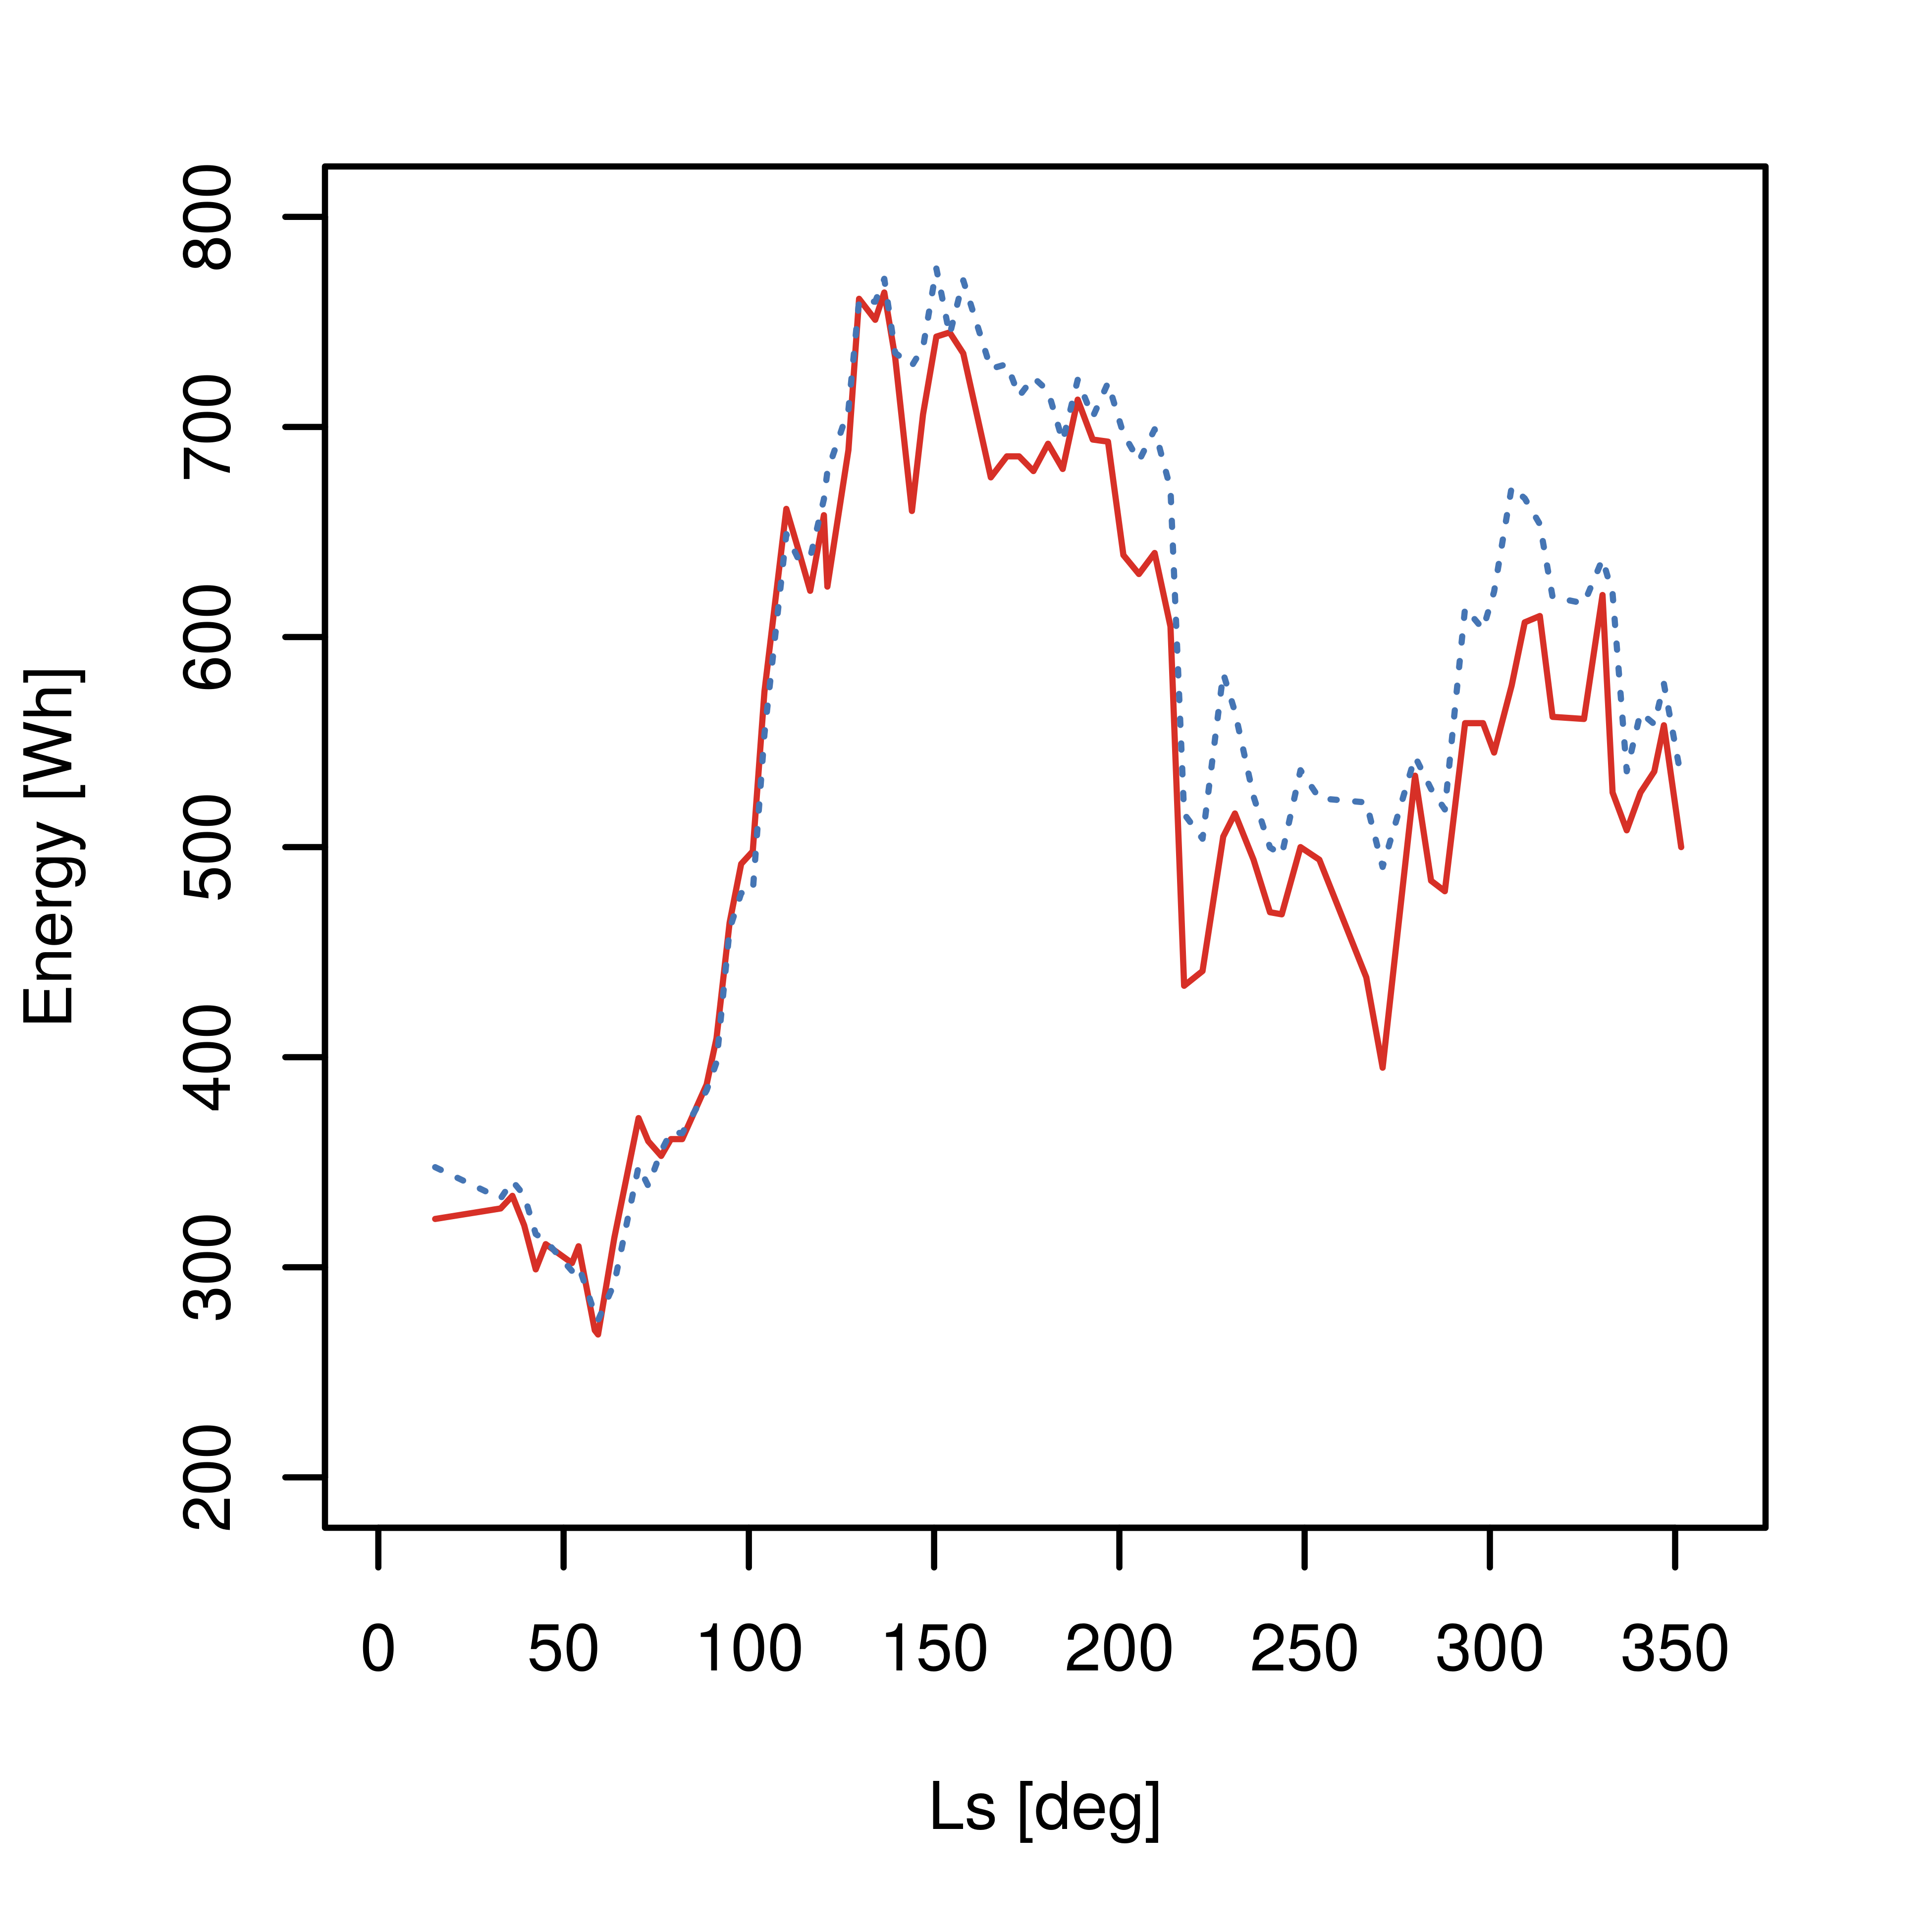
\includegraphics[height=\graphicsHeight]{sections/mars-solar-energy/photovoltaic-energy/plots/predicted-vs-measured-energy-my32.png}
  		\subcaption{MY32}
  		\label{fig:plot:sub:mer-energy-production-predicted-vs-reported-my32}
  	\end{subfigure}\hfill
	   \begin{subfigure}[t]{\subfigureWidth}
      \centering
  		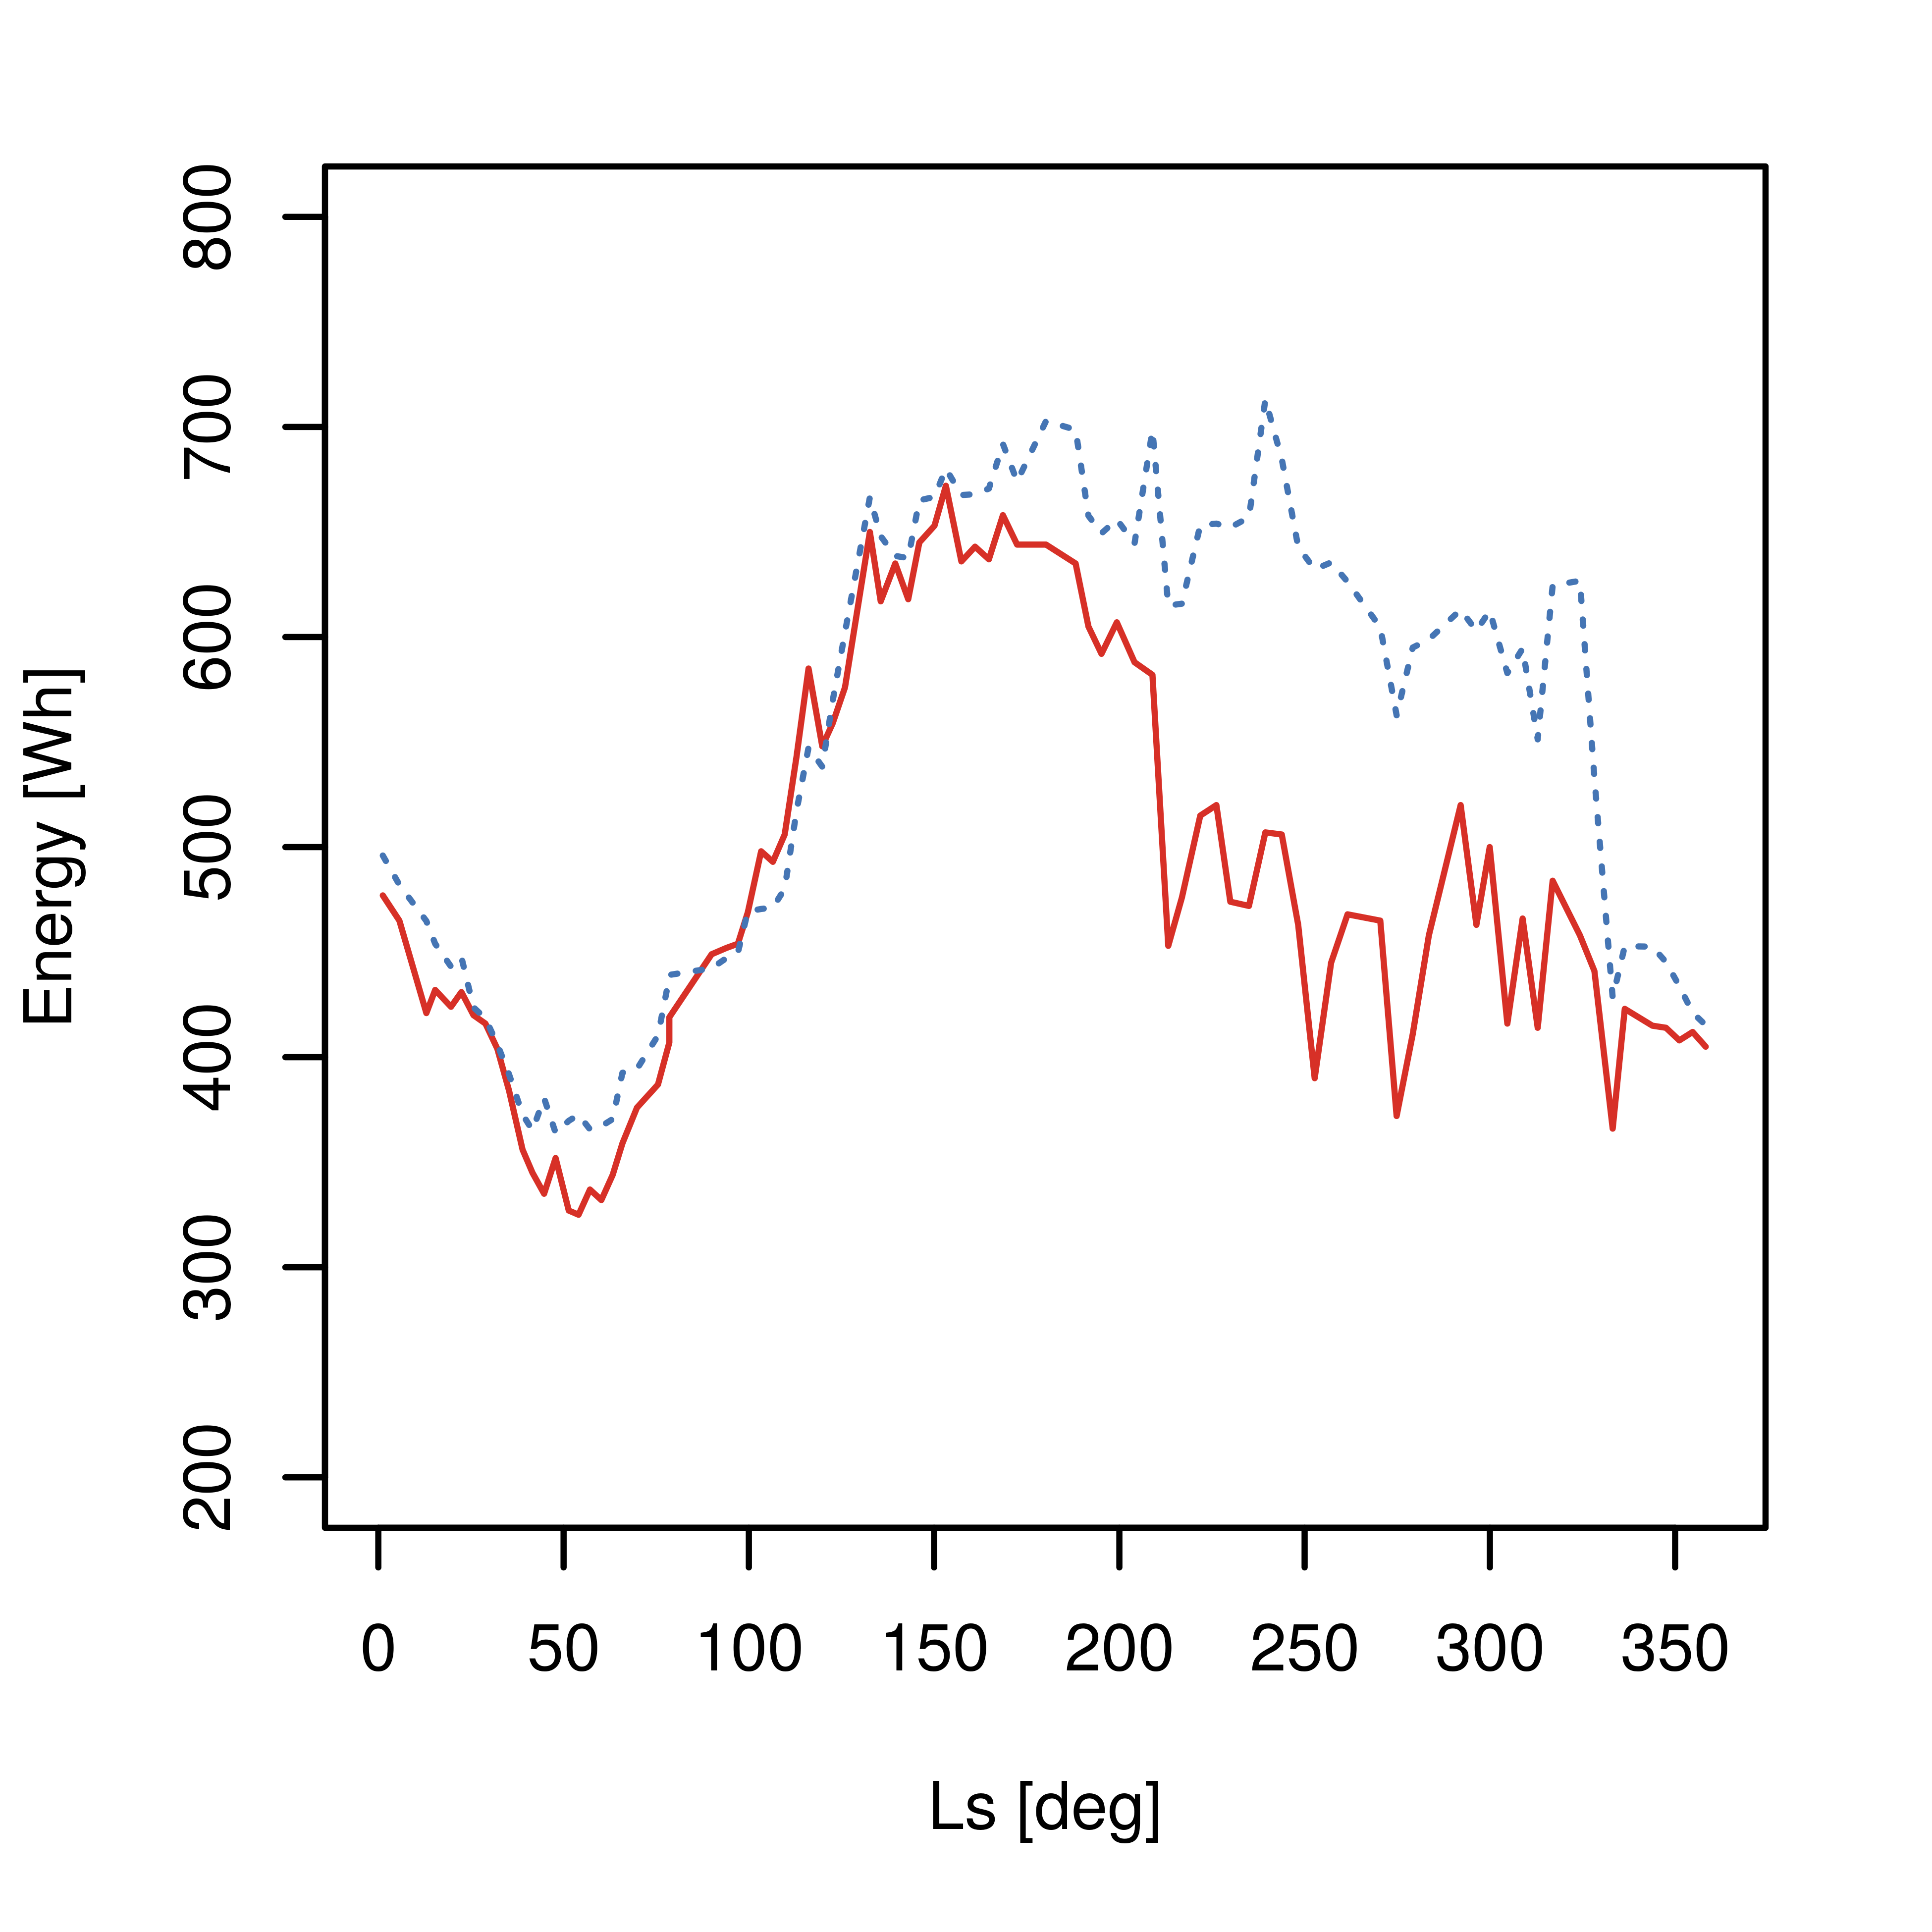
\includegraphics[height=\graphicsHeight]{sections/mars-solar-energy/photovoltaic-energy/plots/predicted-vs-measured-energy-my33.png}
  		\subcaption{MY33}
  		\label{fig:plot:sub:mer-energy-production-predicted-vs-reported-my33}
	   \end{subfigure}\hfill
    \caption[Opportunity energy production: predicted versus reported]
            {Opportunity energy production: predicted versus reported. Not shown are data for \ac{MY}28 and \ac{MY}34 which have also been scraped from the rover's status update logs.}
	\label{fig:plot:mer-energy-production-predicted-vs-reported}
\vspace{-2ex}
\end{figure}

Not included in \refFig{fig:plot:mer-energy-production-predicted-vs-reported} is data for \ac{MY}34 during which the rover spent most of the year driving down ``Perseverance Valley'' on the west rim of Endeavour Crater. As with \ac{MY}33, applying \refEqn{eq:SA_energy} for the \ac{MY}34 would not be appropriate considering the rover's inclination during descents and is not considered in the validation exercise for horizontal surfaces.

Divergences of the measured energy production from those calculated are presented in \refFig{fig:plot:mer-energy-prediction-divergences}. A \SI{-33}{\percent}/+\SI{7}{\percent} error margin range is observed. \refFig{fig:plot:binned-error-margins} bins the distribution of divergences across the \SI{-33}{\percent}/+\SI{7}{\percent} error margin range into \SI{5}{\percent} increments. \SI{65.5}{\percent} of the divergences occur within a \SI{-10}{\percent}/\SI{0}{\percent} error margin and \SI{90.7}{\percent} within \SI{-15}{\percent}/+\SI{5}{\percent}. The wide error margin range is thus a result of isolated local maxima outliers, notably at Sol 2204 (\SI{-33}{\percent}), 2218 (\SI{-27}{\percent}), 2519 (\SI{-28}{\percent}), and 3901 (\SI{-24}{\percent}).

\vspace{1cm}

\begin{figure}[h]
\captionsetup[subfigure]{justification=centering}
\vspace{-2ex}
\centering
    %% setup sizes
    \setlength{\subfigureWidth}{0.50\textwidth}
    \setlength{\graphicsHeight}{80mm}
    %% kill hyper-link highlighting
    \hypersetup{hidelinks=true}%
    %% the figures
    \begin{subfigure}[t]{\subfigureWidth}
        \centering
            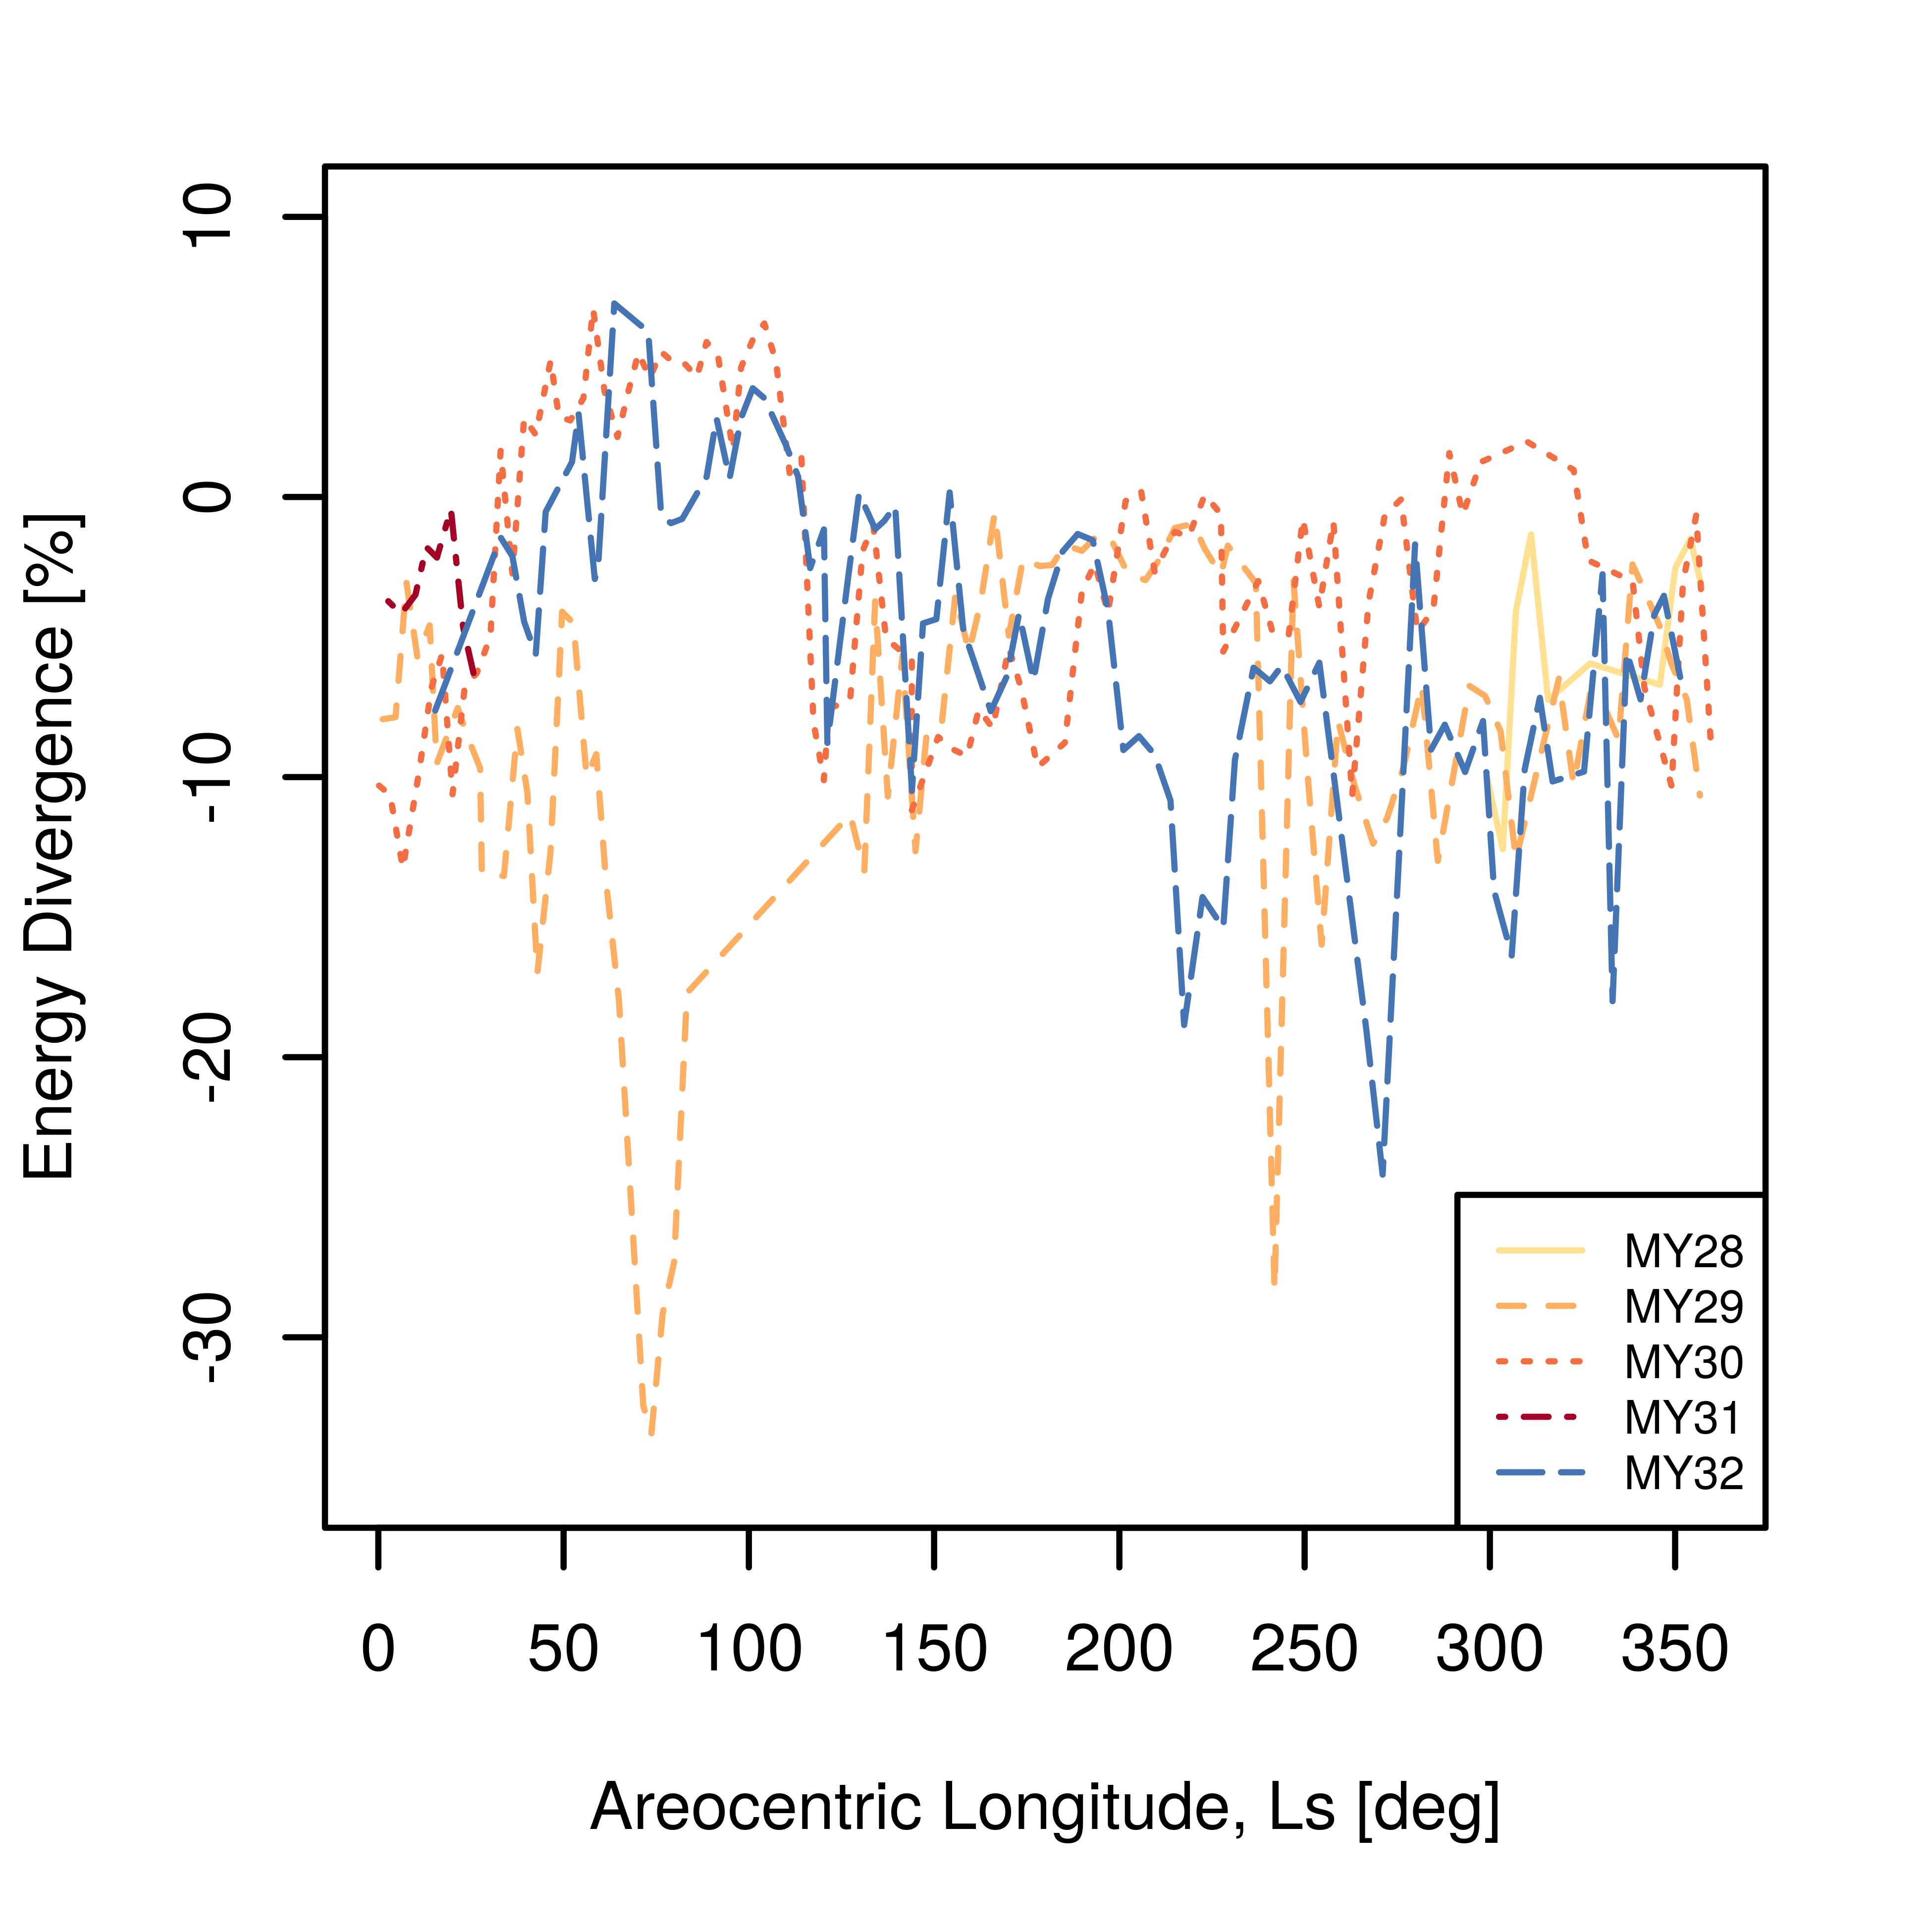
\includegraphics[height=\graphicsHeight]{sections/mars-solar-energy/photovoltaic-energy/plots/energy-prediction-divergences-from-my28-to-my32.png}
            \subcaption{Divergences}
            \label{fig:plot:mer-energy-prediction-divergences}
    \end{subfigure}\hfill
    \begin{subfigure}[t]{\subfigureWidth}
        \centering
            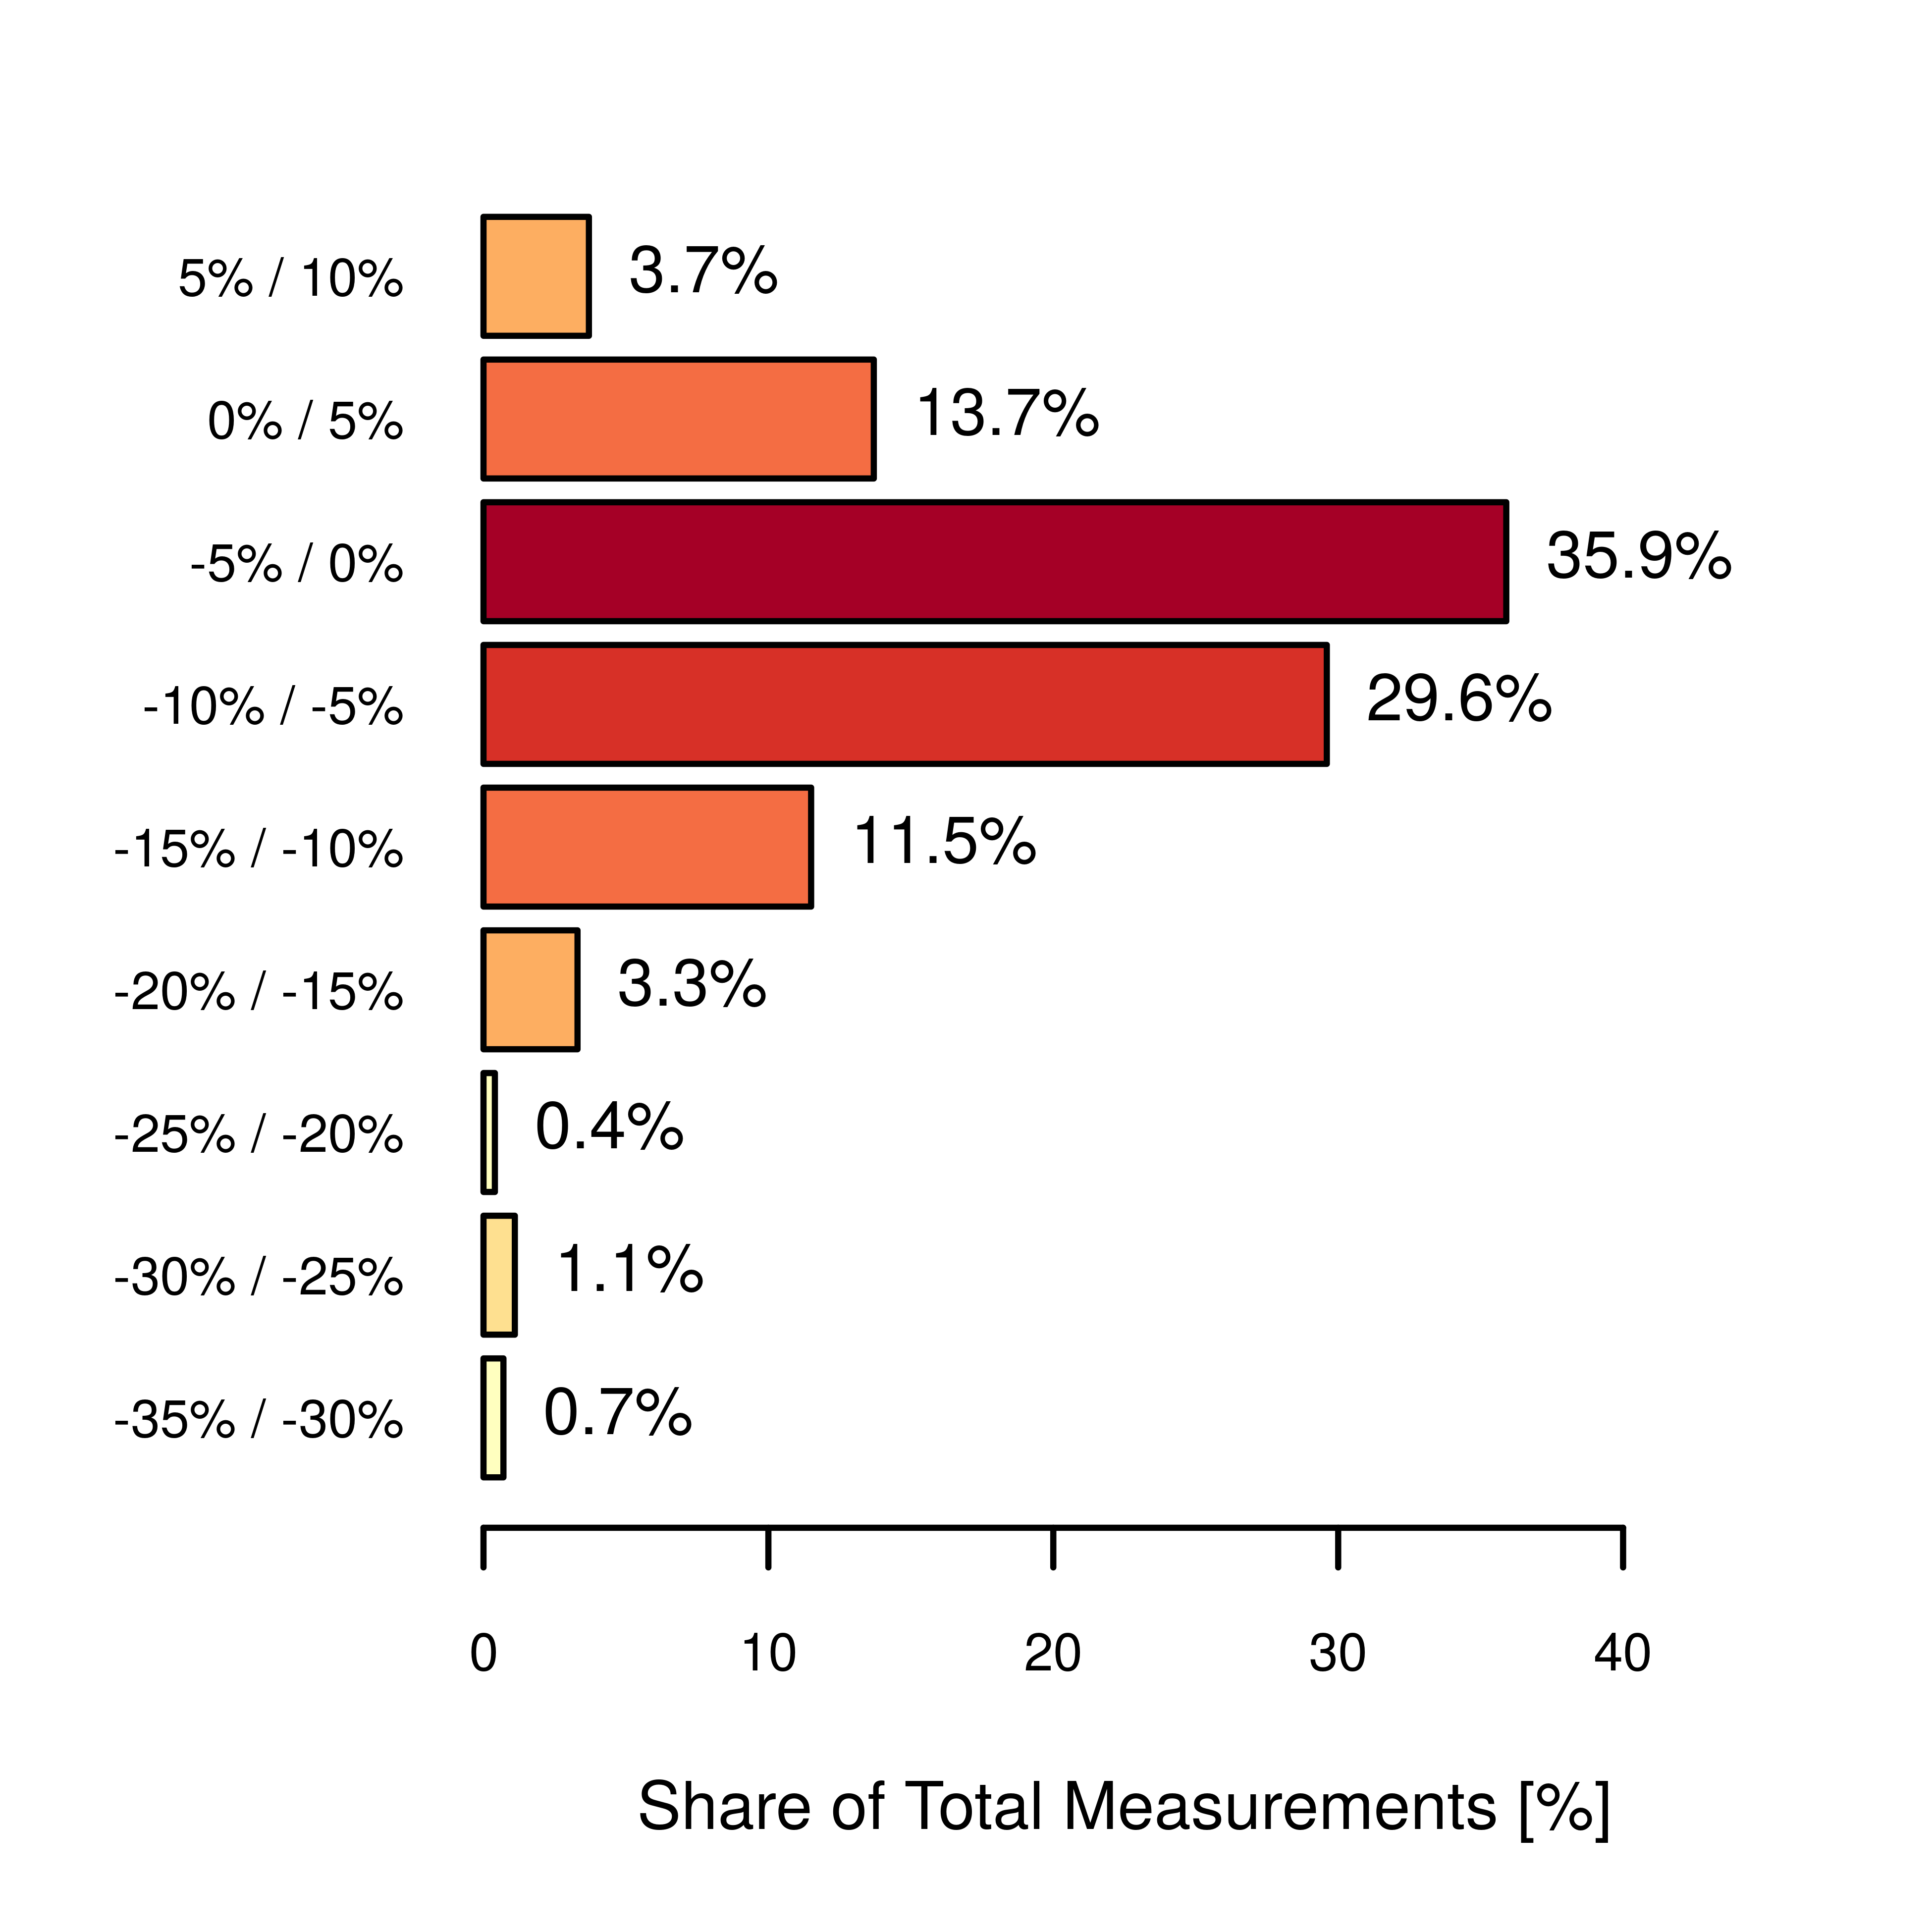
\includegraphics[height=\graphicsHeight]{sections/mars-solar-energy/photovoltaic-energy/plots/binned-error-margins.png}
            \subcaption{Binned error margins}
            \label{fig:plot:binned-error-margins}
    \end{subfigure}\\[0.8ex]
    \caption[Opportunity energy divergences between predicted and reported]
    {Opportunity energy divergences between predicted and reported. Negative values indicate predicted daily energy production greater than what was measured and the inverse is indicated by positive values.}
    \label{fig:plot:energy-divergence}
\vspace{-2ex}
\end{figure}

\vspace{0.5cm}

Divergences that are beyond \SI{-20}{\percent} are listed in \refTab{tab:divergences-less-than-m20pc}.

\begin{table}[h]
    \footnotesize
    \centering
    \caption[Divergences from predicted Opportunity energy production beyond \SI{-20}{\percent}]
        {Divergences from predicted Opportunity energy production beyond \SI{-20}{\percent}.}
    \label{tab:divergences-less-than-m20pc}
    \begin{tabular}{|l|c|c|c|c|c|c|c|}
    \hline
    \multicolumn{1}{|c|}{\multirow{2}{*}{\textbf{Date}}} & \multirow{2}{*}{\textbf{MY}} & \multirow{2}{*}{\textbf{Ls}} & \multirow{2}{*}{\textbf{Sol}} & \multicolumn{4}{c|}{\textbf{Energy [Wh]}} \\ \cline{5-8}
    \multicolumn{1}{|c|}{} &  &  &  & \textbf{Predicted} & \textbf{Measured} & \textbf{Diff.} & \textbf{Diff. [\%]} \\ \hline
    1-APR-2010 & 29 & 72 & 2199 & 315 & 238 & 77 & -32 \\
    6-APR-2010 & 29 & 74 & 2204 & 314 & 235 & 79 & -33 \\
    13-APR-2010 & 29 & 77 & 2211 & 293 & 227 & 66 & -29 \\
    20-APR-2010 & 29 & 80 & 2218 & 314 & 247 & 67 & -27 \\ \hline
    23-FEB-2011 & 29 & 242 & 2519 & 539 & 420 & 119 & -28 \\ \hline
    13-JAN-2015 & 32 & 271 & 3901 & 491 & 395 & 96 & -24 \\ \hline
    \end{tabular}
\end{table}


\vspace{0.5cm}

With the exception of Sol 2199 and 2218, possible explanations for large divergences beyond \SI{-20}{\percent} are obtained from MER Opportunity's status logs:

\begin{enumerate}[label=\textcolor{BulletBlue}{(\alph*)}]
  \item Sol 2199: No turns or inclinations reported.
  \item Sol 2204: Turn - short sharp arc turn.
  \item Sol 2211: Inclination - crossed a series of ripples.
  \item Sol 2218: No turns or inclinations reported.
  \item Sol 2519: Turn - sharp repositioning turn.
  \item Sol 3901: Inclination - descended from the summit of ``Cape Tribulation.''
\end{enumerate}

\vspace{0.5cm}

%\todo[inline]{\textbf{TODO:} Source MER Opportunity status log.}
%Sources. For terrestrial year 2010: https://mars.nasa.gov/mer/mission/rover-status/opportunity/2010/

The use of fixed daily values for the certain irradiance calculation variables also contributes to the observed divergences:

\begin{enumerate}[label=\textcolor{BulletBlue}{(\alph*)}]
  \item A fixed $\tau$ factor does not reflect the continuous changes in atmopheric optical depth.
  \item A fixed solar array dust factor does not reflect the irregularity of dust deposition over the entirety of the solar cell coverage area.
  \item A fixed shadowing performance loss coefficient does not reflect the diurnal changes in overshadowed area. Overshadowing changes throughout the day due to the position of the sun with respect to the location of the rover's petruding instruments, notably the \ac{PMA} as well as the low-gain and high-gain antennas.
\end{enumerate}

Attempts to narrow down the error margin range by adjusting the reported dust factor as well as shadowing and other losses are described in \refApp{sec:Appendix:EnergyErrorMargin}. However, these attempts resulted in overly conservative energy predictions and will not be applied. By setting aside outliers causing divergences greater than \SI{5}{\percent} and lesser than \SI{-15}{\percent} obtained with only \SI{9.2}{\percent} of the dataset, the predicted energy production obtained with \refEqn{eq:SA_energy} becomes acceptable for preliminary mission scenario analysis on a horizontal surfaces.

\subsubsection{Inclined Surface}
\label{sec:PowerAndEnergyPredictions:Validation:InclinedSurface}

\refEqn{eq:SA_slope_energy} for energy predictions on an inclined surface requires slope and rover orientation angles in order to determine $H_{\beta}$. However, these parameters are seldom reported in the \ac{MER} Opportunity status updates. Cherry-picked energy production measurements made while \ac{MER} Opportunity's descent and ascent of Endaveaour crater during \ac{MY}33 is used in an attempt to validate predictions made with \refEqn{eq:SA_slope_energy}. These measurements are selected based on traverse phases that preserved consistent orientations which could be more reliable measured from the rover's Traverse Map Archive \citeother{OpportunityTraverseMapArchive}:

An average slope angle of 13 degrees is assumed based on the following:
\begin{itemize}
  \item On Sol 4269 and 4270, \ac{MER} Opportunity status logs reported that the rover climbed slopes close to \SI{30}{\degree} near the crest of ``Knudsen Ridge'', reaching \SI{32}{\degree} on March 10, 2016 (Sol 4310).
  \item An image taken in March 22, 2016 (Sol 4322), was rotated \SI{13.5}{\degree} degrees to adjust for the tilt of the rover.
  \item Perseverance Valley extends downhill at around \SI{15}{\degree} for about \SI{200}{\meter} toward Endeavour crater's interior.
\end{itemize}

As in \refSec{sec:PowerAndEnergyPredictions:Validation:HorizontalSurface}, performance ratios described in \refSec{sec:PowerAndEnergyPredictions:PerformanceRatio} are also used. Due to large uncertainties regarding slope rover orientation angles, this section only aims to validate that \refEqn{eq:SA_slope_energy} results in smaller energy predictions divergences than what would otherwise be obtained using \refEqn{eq:SA_energy}. The results are presented in \refTab{tab:divergences-inclined-surfaces}.


\begin{table}[h]
\footnotesize
\centering
\caption{Divergences from predicted MER Opportunity PV energy production on inclined surfaces.}
\label{tab:divergences-inclined-surfaces}
\begin{tabular}{|c|c|c|c|c|c|}
\hline
\multicolumn{1}{|l|}{\multirow{3}{*}{\textbf{Sol}}} & \multirow{3}{*}{\textbf{\begin{tabular}[c]{@{}c@{}}Measured\\ Energy\\ {[}Wh{]}\end{tabular}}} & \multicolumn{4}{c|}{\textbf{Predicted Energy}} \\ \cline{3-6}
\multicolumn{1}{|l|}{} &  & \multicolumn{2}{c|}{\textbf{Horizontal Surface}} & \multicolumn{2}{c|}{\textbf{Inclined Surface}} \\ \cline{3-6}
\multicolumn{1}{|l|}{} &  & \multicolumn{1}{l|}{\textbf{$E$ {[}Wh{]}}} & \multicolumn{1}{l|}{\textbf{Diff. {[}\%{]}}} & \multicolumn{1}{l|}{\textbf{$E_{\beta}$ {[}Wh{]}}} & \multicolumn{1}{l|}{\textbf{Diff. {[}\%{]}}} \\ \hline
4493 & 515 & 653 & -27 & 407 & 21 \\ \hline
4582 & 411 & 595 & -45 & 535 & -30 \\ \hline
4623 & 416 & 583 & -40 & 284 & 32 \\ \hline
4630 & 466 & 595 & -28 & 526 & 13 \\ \hline
\end{tabular}
\end{table}


\refEqn{eq:SA_slope_energy} resulted in a larger divergence range than with \refEqn{eq:SA_energy} at \SI{-30}{\percent}/\SI{32}{\percent} for the former and \SI{-45}{\percent}/\SI{-27}{\percent}for the latter. However, the magnitude of divergences are smaller with \refEqn{eq:SA_slope_energy}. Furthermore, with the exception of Sol 4582, divergences with \refEqn{eq:SA_slope_energy} result in conservative under-estimated energy predictions rather than the worst-case over-estimated values consistently obtained with \refEqn{eq:SA_energy}.


The pool of measured data used for this validation is much too small to draw convincing conclusions and the magnitude of divergences remain significantly large. Inaccurate slope and rover orientation angles are likely to have contributed to unfavourable results. Further data must be obtained to validate \refEqn{eq:SA_slope_energy} against reported measurements. %However, for the purpose of this thesis, mission scenario analysis on inclined surfaces will still rely on predictions obtained with \refEqn{eq:SA_slope_energy} in light of it being derived from applying solar geometry to \refEqn{eq:SA_energy}, with which favourably results were obtained as described in \refSec{sec:PowerAndEnergyPredictions:Validation:HorizontalSurface}.

% [z] Rover traverse map. [https://mars.nasa.gov/mer/mission/traverse-maps/opportunity/]
% [a] https://mars.nasa.gov/mer/mission/rover-status/opportunity/recent/all/?y=2016
% [b] https://www.jpl.nasa.gov/news/news.php?feature=6193
% [c] https://www.planetary.org/explore/space-topics/space-missions/mer-updates/2018/04-mer-update-special-perseverance-valley-lpsc-2018.html

%Particularly while it was exploring steep outcrops within 'Marathon Valley' when the rover was inclined on the slopes of 'Knudsen Ridge' at Sol 4303 (March 1, 2016).
%The rover's tilt hit 32 degrees on March 10 while Opportunity was making its closest approach to an intended target near the crest of "Knudsen Ridge."

%\subsection{Summary}
%\todo[inline]{\textbf{TODO:} Write section summary.}
